\documentclass[a4paper]{article}
\usepackage[a4paper, top=17mm, bottom=17mm, left=17mm, right=17mm]{geometry}
\usepackage[utf8]{inputenc}
\usepackage[T2A,T1]{fontenc}
\usepackage[colorlinks,filecolor=blue,citecolor=green,unicode,pdftex]{hyperref}
\usepackage{cmap}
\usepackage[english,russian]{babel}
\usepackage{amsmath}
\usepackage{amssymb,amsfonts,textcomp}
\usepackage{color}
\usepackage{array}
\usepackage{hhline}
\hypersetup{colorlinks=true, linkcolor=blue, citecolor=blue, filecolor=blue, urlcolor=blue, pdftitle=1, pdfauthor=, pdfsubject=, pdfkeywords=}
\usepackage[pdftex]{graphicx}
\usepackage{graphicx}
% \usepackage{epigraph}
% Раскомментировать тем, у кого этот пакет есть. Шрифт станет заметно красивее.
%\usepackage{literat}
\usepackage{indentfirst}
\usepackage{multirow}
\usepackage{subfig}

\sloppy
\pagestyle{plain}
%\pagestyle{empty}

\title{Технология визуального предметно-ориентированного проектирования и разработки ПО QReal}

\author{А.Я.Кириленко \and Наталья Вальтман}
\date{}
\begin{document}

\maketitle
\thispagestyle{empty}

\begin{quote}
\small\noindent
В статье описываеся инструментальная среда QReal, являющаяся как CASE-средством, так и позволяющая быстро создавать визуальные предметно-ориентированные языки, редакторы и генераторы исходных кодов для них. Алсо, слава роботам!
\end{quote}

\section*{Введение}

Модельно-ориентированная разработка ПО (model-driven development, MDD~\cite{mdd}) основывается на представлении программы в виде набора моделей, представляющих ее с различных точек зрения. При этом обычно используются визуальные языки моделирования, с их помощью создаются разного уровня абстракции описания предметной области, разрабатываемой системы и взаимодействующего с ней окружения. Считается, что в целом данный подход упрощает процесс разработки и понимания системы, делает его более наглядным, снижает вероятность появления ошибок, повышает продуктивность разработчиков. Наиболее активное распространение CASE-технологий\footnote{Computer-aided software engineering}  началось в середине 90-х годов прошлого века, когда появился унифицированный язык моделирования UML\footnote{http://www.uml.org/}. К концу 90-х годов был разработан набор методологий разработки ПО (и поддерживающих их инструментариев), в том или ином виде предполагающих активное использование визуального проектирования. Среди них MDA (model-driven architecture\footnote{http://www.omg.org/mda/}), методология ROOM (Real-Time Object-Oriented Modeling~\cite{room}), [моар примеров]. Однако, желание иметь полную автоматическую генерацию исполняемого кода по диаграммам неизбежно влечет к жесткой формализации соответствующих графических языков. При этом использование языков общего назначения (например, Executable UML~\cite{xuml}) чаще всего приводит к тому, что диаграммы теряют наглядность и простоту, становятся громоздкими и сложными для восприятия. Парадигма предметно-ориентированного моделирования (Domain-specific modeling~\cite{theBook}) же основывается на том факте, что чаще создание нового специального языка и решение с его помощью поставленной практической задачи можно осуществить быстрее, чем решать ту же задачу с помощью языков общего назначения. Имея соответствующую инструментальную поддержку, данный подход позволяет значительно повысить уровень абстракции, но котором работают проектировщики, и увеличить производительность их труда в несколько раз ~\cite{dsm01, dsm02, dsm03}.

\section{Предыстория}

Разработкой технологии QReal занимается научно-исследовательская группа изучения технологий визуального моделирования кафедры системного программирования Санкт-Петербургского Государственного Университета. Проект QReal базируется на результатах, полученных на кафедре и в лаборатории системного программирования под руководством проф. А.Н. Терехова с 1984 года. Первые разработанные графические редакторы создавались для поддержки языка SDL (Specification and Description Language, рекомендация МККТТ Z.100 ~\cite{sdl}), к концу 80-х годов была реализована генерация программ управления телефонными станциями, генерация баз данных и сложных форм ввода/вывода к ним — технология RTST~\cite{rtst}. 

К середине 90-х годов группой была реализована поддержка появившегося в то время языка UML 1.4 в виде технологии REAL~\cite{real}. Технология не создавалась как универсальная, а была ориентирована на создание информационных систем, ориентированных на данные (диаграммы классов, объектов, задание ограничений с помощью OCL\footnote{Object Constraint Language}), а также создания встроенных систем реального времени (диаграммы классов, последовательностей, конечных автоматов). 

Технология QReal~\ref{qreal}  изначально задумывалась как развитие технологии REAL, основывающееся на использовании более современной версии языка UML --- 2.0. При этом на разрабатываемые средства накладывались требования многоплатформенности (возможность работы на наиболее популярных операционных системах MS Windows и Linux), поддержка многопользовательской разработки, возможность удаленного доступа к репозиторию системы и другая актуальная для сред визуального проектирования ПО функциональность. Однако, очевидно, что создание большого числа редакторов диаграмм вручную является довольно утомительным занятием, к тому же получаемая система оказывается плохо масштабируемой --- создание дополнительного редактора, являющегося типовым для данного CASE-средства, чаще всего будет осуществляться методом Copy/Paste с дальнейшими доработками полученного после копирования, что влечет как к появлению дополнительных ошибок, связанных с неполнотой вносимых правок, так и к размножению уже существующих. В результате в QReal были добавлены средства метамоделирования, которые позволяют быстро создавать новые редакторы, описывания метамодель разрабатываемого языка и визуальное представление его элементов.

\section{QReal}

\subsection{Архитектура}
Инфраструктуру QReal можно представить следующим образом (см. рис.~\ref{qRealArchitecture}):

\begin{itemize}
  \item Архитектура QReal основывается на шаблоне проектирования Model/View. Модель обеспечивает доступ к репозиторию, а в роли представлений выступают различные элементы пользовательского интерфейса (инспектор логических и графических моделей, редактор свойств и т.д.). Графический интерфейс QReal обычно содержит вполне определенный набор элементов: инспектор логических моделей, инспектор графических моделей, редактор свойств элементов, палитра компонентов, окно отображения ошибок и предупреждений, различные меню, панели инструментов, рабочая область графических редакторов диаграмм.
  \item Ввиду того, что набор графических редакторов QReal не фиксирован, каждый визуальный редактор является подключаемым модулем. Инфраструктура CASE-системы включает в себя абстрактное ядро, реализующее общую для всех редакторов и элементов диаграмм функциональность, и подключаемых модулей, реализующих специфику конкретных редакторов. Каждый такой модуль инкапсулирует в себе информацию о наборе объектов, допустимых на диаграммах данного типа, позволяет правильно интерпретировать хранящиеся в репозитории значения атрибутов элементов (например, использовать некоторые из атрибутов как параметры при отрисовке элементов), предоствляет информацию о логических правилах размещения элементов на соответствующих типах диаграмм (например, возможность соединять некоторые элементы ассоциациями, возможность одних элементов быть контейнером для других и т.д.).
\begin{figure} [ht]
  \begin{center}
    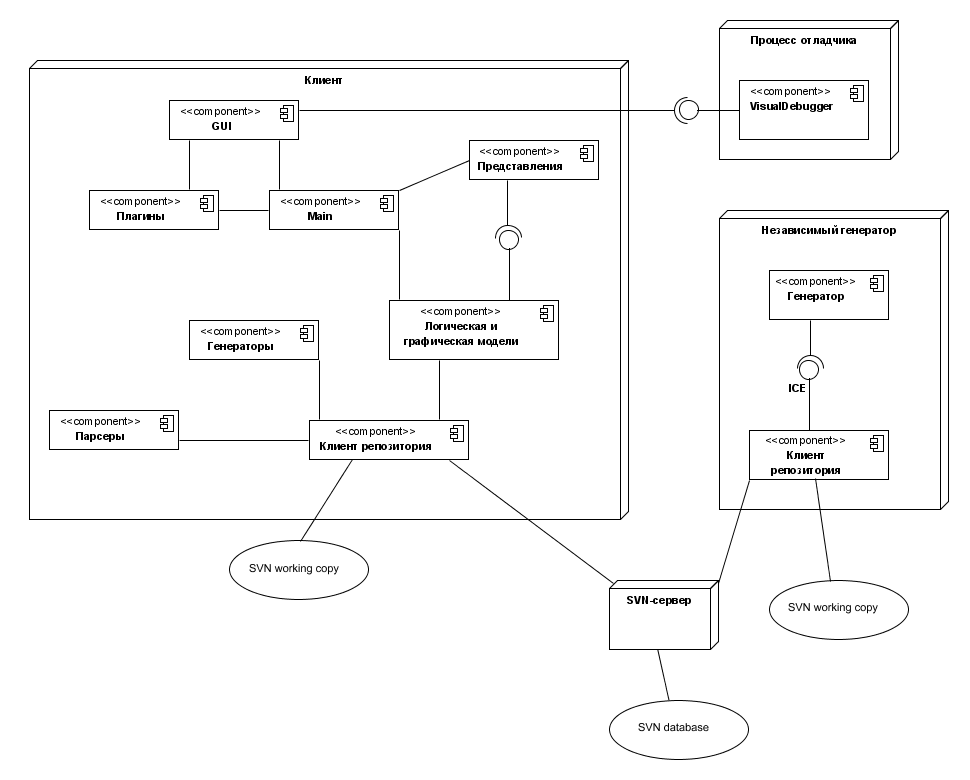
\includegraphics[width=0.9\textwidth]{01-architecture.png}
    \caption{Архитектура QReal}
    \label{qRealArchitecture}
  \end{center}
\end{figure}
  \item Для обеспечения версионирования и многопользовательской работы используется сервер Subversion. Доступ к нему осуществляется посредством клиентов репозитория, которые хранят свои модели в виде файлов, организованных в рабочую копию системы контроля версий. При старте QReal файлы моделей читаются с диска и строится особая объектная структура, с которой и происходит работа при манипуляциями с репозиторием. При выходе из системы (либо по запросу пользователя) содержимое клиента репозитория может быть сериализовано на диск и внесенные изменения отправляются на SVN-сервер. В настоящее время в QReal поддержаны основные команды работы с subversion: commit, checkout, update. 
  \item Генераторы могут быть встроенными в клиентскую часть CASE-пакета (например, генератор XMI-описаний диаграмм [ссылка]) или работать независимо. В таком случае им потребуется компонента, отвечающая за взаимодействие с SVN-репозиторием и представление модели в памяти. Общение с ней ведётся по протоколу ICE~\ref{ice}, что позволяет реализовывать генераторы на различных языках программирования.
\item Основная идея разделения логических и графических моделей состоит в том, что элемент модели и его визуальное представление --- по сути разные вещи. Некоторые элементы модели могут вовсе визуального представления не иметь (например, значения перечислимых типов или специальные служебные вещи типа настроек генерации), некоторые наоборот, имеют только визуальное представление и на логику никак не влияют (например, просто линия или прямоугольник на диаграмме), некоторые могут иметь несколько представлений (например, один и тот же класс UML может присутствовать на нескольких разных диаграммах, причём выглядеть по-разному). 
\end{itemize}


\subsection{Средства метамоделирования}

В QReal реализованы два подхода, позволяющие любому заинтересованному пользователю системы, не обладающему навыками программирования и не знакомому с внутренним устройством системы, создать новый редактор диаграмм, встраивающийся в QReal.
\begin{itemize}
  \item Метамодель разрабатываемого языка описывается в виде XML-формата довольно простой структуры. Графические изображения элементов задаются с помощью текстового языка SDF, являющегося расширением языка описания векторной графики SVG~\footnote{Scalable Vector Graphics, http://www.w3.org/Graphics/SVG/}.
  \item Метамодель языка задается графически в метаредакторе QReal последством простого визуального языка, являющего аналогом MOF~\footnote{MetaObject Facility, http://www.omg.org/mof/}. Для описания представлений элементов языка на диаграммах используется графический редактор форм, позволяющий создавать из набора примитивов векторные изображения или загружать уже готовые растровые.
\end{itemize}
Эти два подхода являются взаимозаменяемыми, поскольку XML-описание метамодели языка может быть как загружено в метаредактор, так и сгенерировано из него. 

В дополнение к метаредактору для быстрого создания трансляторов визуальных диаграмм в исходный код на некотором текстовом языке в QReal используется специальный язык описания генераторов. Так, для каждого разрабатываемого визуального языка можно задать правила обхода созданных с его помощью диаграмм и генерации кода. В дальнейшем эти правла интерпретируются для конкретных диаграмм, порождая соответствющий им код на целевом языке.
  
\subsection{Отладчик}

Для редактора блок-схем и некоторых других основанных поведенческих диаграммах, основывающихся на сетях петри, в QReal реализован визуальный интерпретатор, который позволяет разработчику пошагово выполнять созданные диаграммы. При этом среда на каждом шаге автоматически проверяет синтаксическую и семантическую корректность созданной диаграммы, текущий элемент или связь подсвечиваются. Стоит отметить, что разработчик может менять диаграмму прямо в процессе интерпретации, что дает дополнительные удобства для отладки созданных алгоритмов. 
  
Помимо пошаговой интерпретации, в QReal ведется работа и над полноценной отладкой сгенерированного по диаграммам исполнимого кода. Для каждого типа используемых целевых отладчиков (gdb для С/C++, pdb для Python и др.) в QReal создается отдельный модуль, реализующий общий для всех абстрактный интерфейс отладчика, предоставляющий системе запускать программу, выполнять пошаговую отладку, устанавливать точки останова, завершать процесс и т.д. Выполняя поданные команды, модуль отладчика сообщает о результатах обратно в QReal, передавая дополнительную информацию типа текущих значений переменных (watch list), [???] и др. 
  
\subsection{Advanced usability}

Большое значение в QReal уделяется удобству и простоте использования инструментальных средств (usability). Так, был реализован подход, при которым создание объектов на диаграммах и связей между ними ассоциируется с определёнными жестами мышью (в общем случае каждому элементу ставится в соответствие отдельный жест), выполненный с каким-либо модификатором (в случе QReal --- с зажатой правой кнопкой мыши). При выполнении жеста в укзанном месте диаграммы создается соответствующий объект. Например, если пользователь на диаграмме случаев использования UML рисует круг, у него создаётся случай использования (use case), если рисует актёра --- создаётся элемент ``актёр'' (actor). На наш взгляд данный механизм позволяет автоматизировать и ускорить наиболее часто выполняемые при проектировании диаграмм операции --- создание и удаление элементов. Также в процессе моделирования важным является удобство работы с связями между элементами. В QReal точки излома ассоциаций можно добавить, просто потащив за какой-либо участок ломаной. При выделении объекта на диаграмме вокруг него появляются несколько разноцветных кружков, каждый из которых ассоциирован с видами связей, которые из данного элемента могут исходить. При нажатии на эти кружки из элемента можно “вытащить” связь. Если пользователь при этом отпускает кнопку мыши на свободном пространстве диаграммы, ему предлагается список элементов, которых можно соединить с выбранным данным типом связи. Если же кнопка мыши отпускается на существующем элементе, система проверяет, можно ли соединить эти элементы выбранным типом связи, и решает, стоит ли создавать данную ассоциацию или нет. 

\section{Заключение}

Описанный в статье metaCASE инструментарий QReal был использован для создания ряда визуальных редакторов и генераторов исходного кода по ним: набор редакторов UML 2.1 (с генерацией в Java и C\#.NET), редактор бизнес-процессов на язке BPEL, редактор требований, ряд предметно-ориентированных решений для описания схем FPGA, интернет-сервисов для платформы Android, программ, распараллеливаемых с помощью MPI и др.

\begin{thebibliography}{9001}
  \bibitem{qreal} А.Н. Терехов, Т.А. Брыксин, Ю.В. Литвинов и др., Архитектура среды визуального моделирования QReal. // Системное программирование. Вып. 4. СПб.: Изд-во СПбГУ. 2009, С. 171-196
  \bibitem{rtst} В.В. Парфенов, А.Н. Терехов. RTST - технология программирования встроенных систем реального времени. // Системная информатика. Новосибирск. 1997. N5. C. 228-256
  \bibitem{real} Терехов А.Н., Романовский К.Ю., Кознов Д.В. и др. REAL: методология и CASE-средство для разработки систем реального времени и информационных cистем // Программирование. 1999. № 5. C. 44-52.
  \bibitem{mdd} Schmidt, D. Model-Driven Engineering // IEEE Computer, Vol. 39, No. 2. 2006. p. 25-31. URL: http://www.cs.wustl.edu/\textasciitilde schmidt/PDF/GEI.pdf
  \bibitem{room} Selic, B., Gullekson, G., Ward, P. T. Real-Time Object-Oriented Modeling // John Wiley \& Sons. 1994. 560 pp.
  \bibitem{xuml} Mellor, S. J., Balcer, M. J., Executable UML: A Foundation for Model-Driven Architecture // Addison-Wesley. 2002. 416 pp.
  \bibitem{theBook} Kelly, S., Tolvanen, J. Domain-Specific Modeling: Enabling Full Code Generation // Wiley-IEEE Computer Society Press. 2008. 448 pp.
  \bibitem{dsm01} Kelly, S., Tolvanen, J.-P. Visual domain-specific modeling: benefits and experiences of using metaCASE tools // Proceedings of International workshop on Model Engineering, ECOOP 2000, 
  \bibitem{dsm02} Weiss, D., Lai, C.T.R. Software Product-Line Engineering: A Family-Based Software Development Process // Addison Wesley, Longman, 1999, 448 pp.	
  \bibitem{dsm03} Kieburtz, R. et al. A software engineering experiment in software component generation // Proceedings of 18th International Conference on Software Engineering. Berlin, IEEE Computer Society Press. 1996
  \bibitem{sdl} Specification and description language (SDL). ITU-T Z.100. URL: http://www.itu.int/ITU-T/studygroups/com10/languages/Z.100\_1199.pdf
  \bibitem{ice} The Internet Communications Engine, ZeroC Inc., 2009, URL: http://www.zeroc.com/ice.html.

\end{thebibliography}

\end{document}